\documentclass[11pt]{article}
\usepackage{geometry}
\usepackage{graphicx}
\usepackage{hyperref}
\geometry{a4paper, margin=1in}
\title{MyInfArith:Infinite Precision Calculator}
\author{Aryan Agarwal\\Roll Number: ES23BTECH11008\\GitHub : AryanAg2701}
\date{\today}

\begin{document}
\maketitle

\section{Introduction}
In this project, I built a Java tool called \texttt{MyInfArith} that can do math on very big numbers bigger than standard Java types allow. It can add, subtract, multiply, and divide integers and floating-point numbers of any size. I use strings to store the numbers inside the program.

\section{Project Layout}
Here are the main files in the project:
\begin{itemize}
  \item \texttt{MyInfArith.java}: The main program. It reads your inputs and runs the right calculations.
  \item \texttt{AInteger.java}: A class for doing math on big integers.
  \item \texttt{AFloat.java}: A class for doing math on big decimals.
  \item \texttt{build.xml}: An Ant script that helps you compile, package, and run the code.
  \item \texttt{run\_build.py}: A small Python script that calls Ant commands for you.
  \item \texttt{DockerFile}: A small DockerFile which contains list of instructiond to use a Docker image.
\end{itemize}

\section{How It Works}
Both \texttt{AInteger} and \texttt{AFloat} store numbers in two parts:
\begin{itemize}
  \item \texttt{String digits}: The number's digits, without the sign or decimal point.
  \item \texttt{boolean negative}: A flag saying whether the number is negative.
\end{itemize}

When you call methods like \texttt{add}, \texttt{sub}, \texttt{mul}, or \texttt{div}, they handle the sign first, then call helper functions that do the actual digit-by-digit math on the strings.

\section{Building and Running}
\subsection{Using Ant}
I use Apache Ant to automate everything. The \texttt{build.xml} file has these targets:
\begin{itemize}
  \item \texttt{clean}: Deletes previous build files.
  \item \texttt{compile}: Compiles all the Java files.
  \item \texttt{jar}: Packages the compiled classes into \texttt{dist/MyInfArith.jar}.
  \item \texttt{run}: Runs the program with your inputs.
\end{itemize}

To build and run in one step, just type:
\begin{verbatim}
ant run -Dargs="int add 123 456"
\end{verbatim}

\subsection{Using the Python Script}
If you prefer Python, you can also do:
\begin{verbatim}
python3 run_build.py --args "float mul 3.14 2.5"
\end{verbatim}
This runs clean, compile, jar, and run for you.

\section{Using the Program}
First, compile the Java source files directly:
\begin{verbatim}
javac aribtraryarithmetic/*.java
javac MyInfArith/*.java

\end{verbatim}

Then run the main class from the build directory without a JAR:
\begin{verbatim}
java MyInfArith <type> <operation> <num1> <num2>
\end{verbatim}

\noindent Where:
\begin{itemize}
  \item \textbf{type}: \texttt{int} or \texttt{float}
  \item \textbf{operation}: \texttt{add}, \texttt{sub}, \texttt{mul}, or \texttt{div}
  \item \textbf{num1}, \textbf{num2}: Your numbers as strings (e.g., "12345678901234567890").
\end{itemize}

\section{Special Cases}
\subsection{Integers}
If you divide and there's a remainder, I just drop the decimal part (like integer division).

\subsection{Floats}
If you type numbers like ".89" or "83.", I convert them to "0.89" or "83.0" automatically.

\section{Internal Classes}
    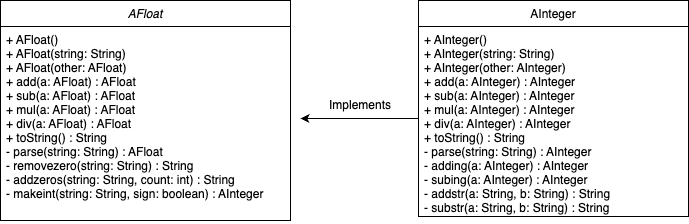
\includegraphics[width=0.8\textwidth]{images/uml.png}
    \\
This section explains the two core classes that power all computations: \texttt{AInteger} for integer math and \texttt{AFloat} for decimal math. Each class stores numbers as strings, handling the sign separately to simplify arithmetic logic.

\subsection{AInteger}
The \texttt{AInteger} class is responsible for handling integer values of arbitrary length. Internally, it stores all digits as a string and the sign as a boolean. This design allows precise control over every digit and mimics manual arithmetic operations at the string level.

\textbf{Fields:}
\begin{itemize}
  \item \texttt{String digits}: Contains the digits of the number as a plain string, without signs or formatting.
  \item \texttt{boolean negative}: True if the number is negative, false otherwise.
\end{itemize}

\textbf{Constructors:}
\begin{itemize}
  \item \texttt{AInteger()}: Initializes the number to 0 with a positive sign.
  \item \texttt{AInteger(String s)}: Parses a string. If it starts with '-', sets negative = true. It also trims any leading zeros.
  \item \texttt{AInteger(AInteger other)}: Creates a deep copy of another \texttt{AInteger}.
\end{itemize}

\textbf{Key Methods:}
\begin{itemize}
  \item \texttt{add(AInteger other)}:
    \begin{itemize}
      \item If the signs differ, converts the operation into subtraction.
      \item If signs match, uses \texttt{addStr(String a, String b)}:
        \begin{itemize}
          \item Pads the shorter string with zeros to match length.
          \item Adds digits from right to left, storing carry.
          \item Reverses and trims the result.
        \end{itemize}
    \end{itemize}
  \item \texttt{sub(AInteger other)}:
    \begin{itemize}
      \item If signs differ, delegates to \texttt{add}.
      \item If signs match, calls \texttt{subStr(String a, String b)}:
        \begin{itemize}
          \item Compares magnitudes to decide which number to subtract from which.
          \item Performs digit-by-digit subtraction with borrow if needed.
        \end{itemize}
    \end{itemize}
  \item \texttt{mul(AInteger other)}:
    \begin{itemize}
      \item Uses \texttt{mulStrByDigit(String a, char d)} to multiply the number by each digit of the other.
      \item Shifts the intermediate result based on position.
      \item Accumulates with \texttt{addStr}.
      \item Sign is negative if exactly one input is negative.
    \end{itemize}
  \item \texttt{div(AInteger other)}:
    \begin{itemize}
      \item Uses \texttt{divStr(String a, String b)} to perform long division.
      \item Builds the quotient digit by digit.
      \item Discards remainder to stay consistent with integer division behavior.
    \end{itemize}
  \item \texttt{static parse(String s)}:
    \begin{itemize}
      \item Cleans and validates the input string.
      \item Returns a new \texttt{AInteger} instance with the parsed digits and sign.
    \end{itemize}
  \item \texttt{toString()}:
    \begin{itemize}
      \item Converts the stored fields back to a user-readable format.
      \item Prepends '-' if negative.
    \end{itemize}
\end{itemize}

\subsection{AFloat}
The \texttt{AFloat} class is designed for handling decimal numbers with arbitrary precision. It extends \texttt{AInteger}'s logic by introducing a decimal position field, allowing accurate arithmetic operations even on large or very small float values.

\textbf{Fields:}
\begin{itemize}
  \item \texttt{String digits}: Stores all digits as a string, removing the decimal point for simplified operations.
  \item \texttt{boolean negative}: Indicates the sign of the number.
  \item \texttt{int dec}: Tells how many digits are present after the decimal point.
\end{itemize}

\textbf{Constructors:}
\begin{itemize}
  \item \texttt{AFloat()}: Initializes the value to zero with dec = 0.
  \item \texttt{AFloat(String s)}:
    \begin{itemize}
      \item Parses strings like "-12.34", splitting at the decimal point.
      \item Combines digits into a single string (e.g., "12.34" becomes "1234" with dec 2).
      \item Handles corner cases like ".75" or "83." by prepending or appending zeros.
    \end{itemize}
  \item \texttt{AFloat(AFloat other)}: Creates a deep copy, copying digits, sign, and dec.
\end{itemize}

\textbf{Key Methods:}
\begin{itemize}
  \item \texttt{add(AFloat other)} and \texttt{sub(AFloat other)}:
    \begin{itemize}
      \item Normalize both numbers to the same dec by adding trailing zeros to the smaller one.
      \item Convert both to their integer form and apply \texttt{AInteger}'s add/sub.
      \item The result's dec remains consistent with the inputs.
    \end{itemize}
  \item \texttt{mul(AFloat other)}:
    \begin{itemize}
      \item Multiplies integer forms using \texttt{AInteger}'s multiplication logic.
      \item Sets result's dec as the sum of both operand scales.
    \end{itemize}
  \item \texttt{div(AFloat other)}:
    \begin{itemize}
      \item Scales both operands to eliminate decimal points.
      \item Multiplies numerator by a power of 10 (e.g., 10\textasciicircum{}1000) for precision.
      \item Uses \texttt{AInteger.div} to get result and sets dec to fixed precision (e.g., 1000).
    \end{itemize}
  \item \texttt{static parse(String s)}:
    \begin{itemize}
      \item Validates that input is a properly formatted float.
      \item Handles inputs like ".007" by adjusting dec and digit string.
    \end{itemize}
  \item \texttt{toString()}:
    \begin{itemize}
      \item Converts back to readable format by placing the decimal at the correct position.
      \item Adds leading/trailing zeros where necessary and adds "-" if the number is negative.
    \end{itemize}
\end{itemize}
\section{Challenges and Edge Cases}
In developing \texttt{AFloat} and \texttt{AInteger}, several issues required special attention to prevent bugs and unexpected behavior. Below are key challenges and the code strategies used to address them.

\subsection*{1. Handling Leading and Trailing Zeros}
When parsing input strings or doing arithmetic, it's important to remove unnecessary zeros, such as "000123" or "123.45000". This avoids incorrect magnitude or floating point misalignment.



\subsection*{2. Parsing Floats with Missing Whole or Decimal Parts}
Users might input floats as ".89", "83.", or "000.0050". These cases are handled in the constructor of \texttt{AFloat}:


\subsection*{3. Avoiding String Index Errors in Division}
When performing string division, it’s easy to get \texttt{StringIndexOutOfBoundsException} if you don’t check lengths. The \texttt{divStr} method ensures we only read valid positions:

\subsection*{4. Overriding \texttt{toString()} for Clean Output}
For both \texttt{AInteger} and \texttt{AFloat}, overriding \texttt{toString()} ensures formatted, human-readable output:
\texttt{AInteger}:

\texttt{AFloat}:
\subsection*{5. Ensures correct digit alignment} By padding the shorter number with leading zeros so both strings are of equal length. This guarantees that digits are added in the correct column positions.



\section{Limitations}
I can handle very large numbers, but limited by available memory and Java's \texttt{String} size. Floats are precise up to 1000 decimal places which can be changed according to choice. If you give inputs in wrong format answer moght be wrong.

\section{Testing}
I tested with random inputs from online generators and compared results with standard calculators. I tried big numbers, zeros in weird spots (like "000123"), and different decimal formats.

\section{Version Control}
I used Git for version control. Below is a placeholder for the commit history diagram:
\begin{figure}[h]
  \centering
  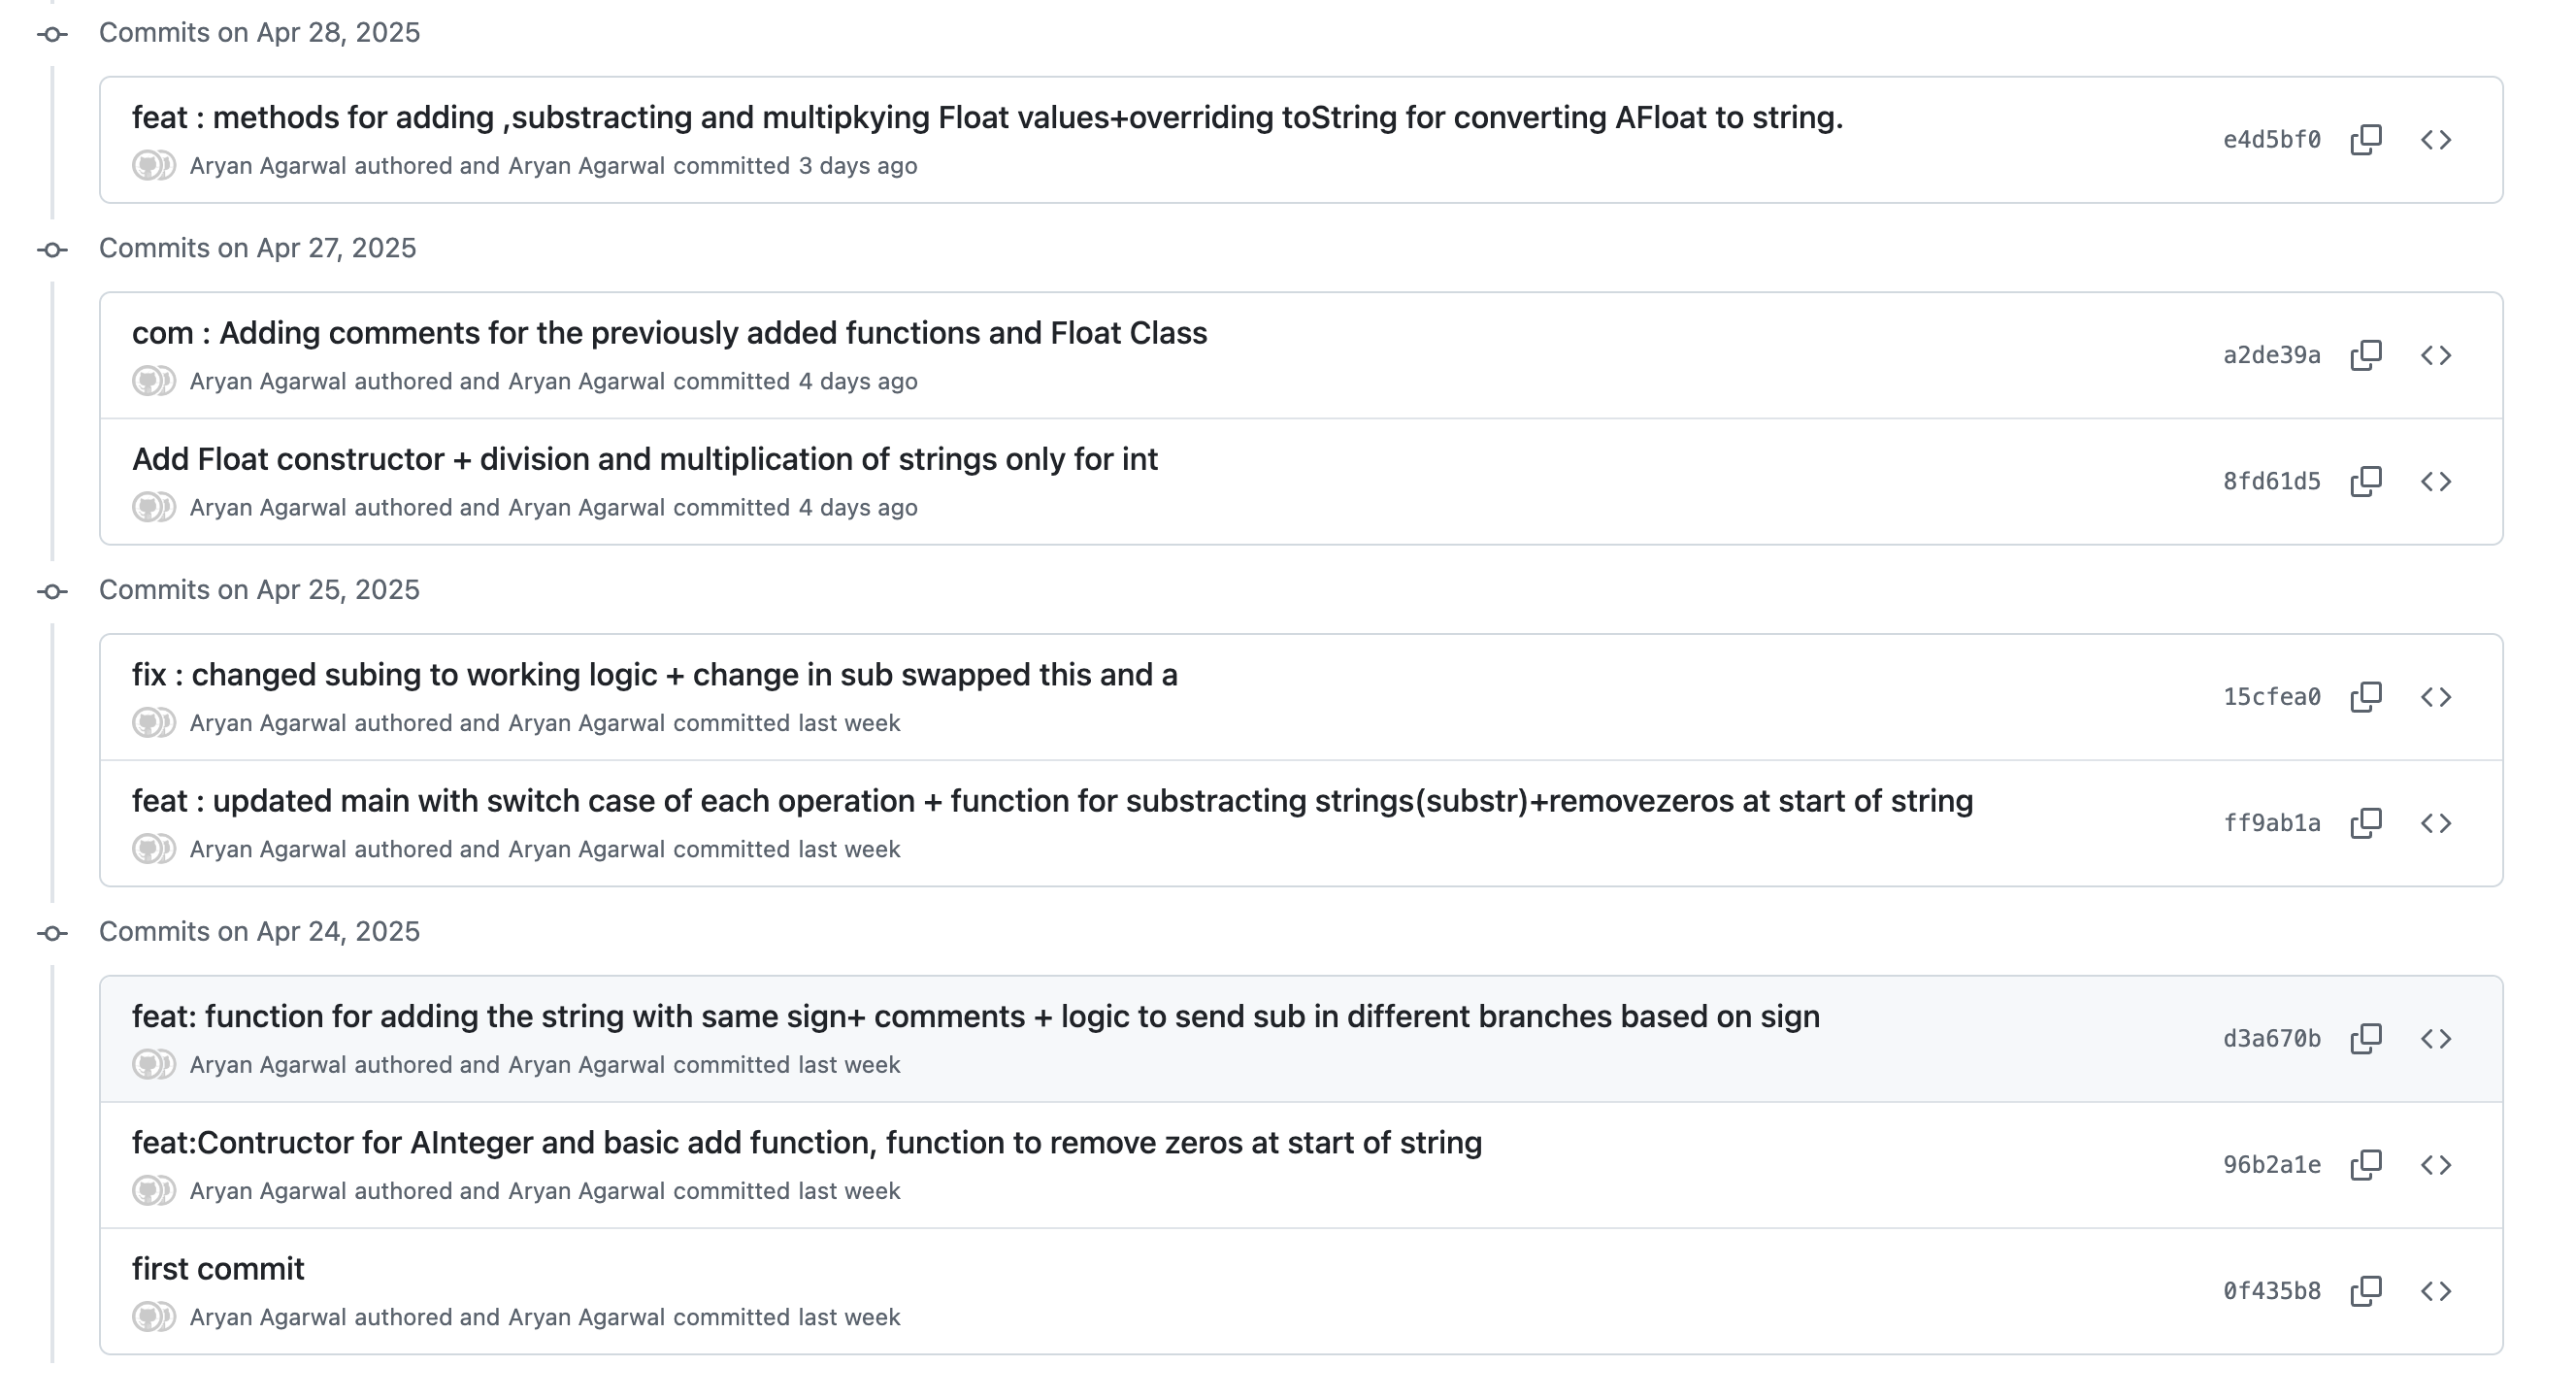
\includegraphics[width=0.8\textwidth]{images/p1.png}
    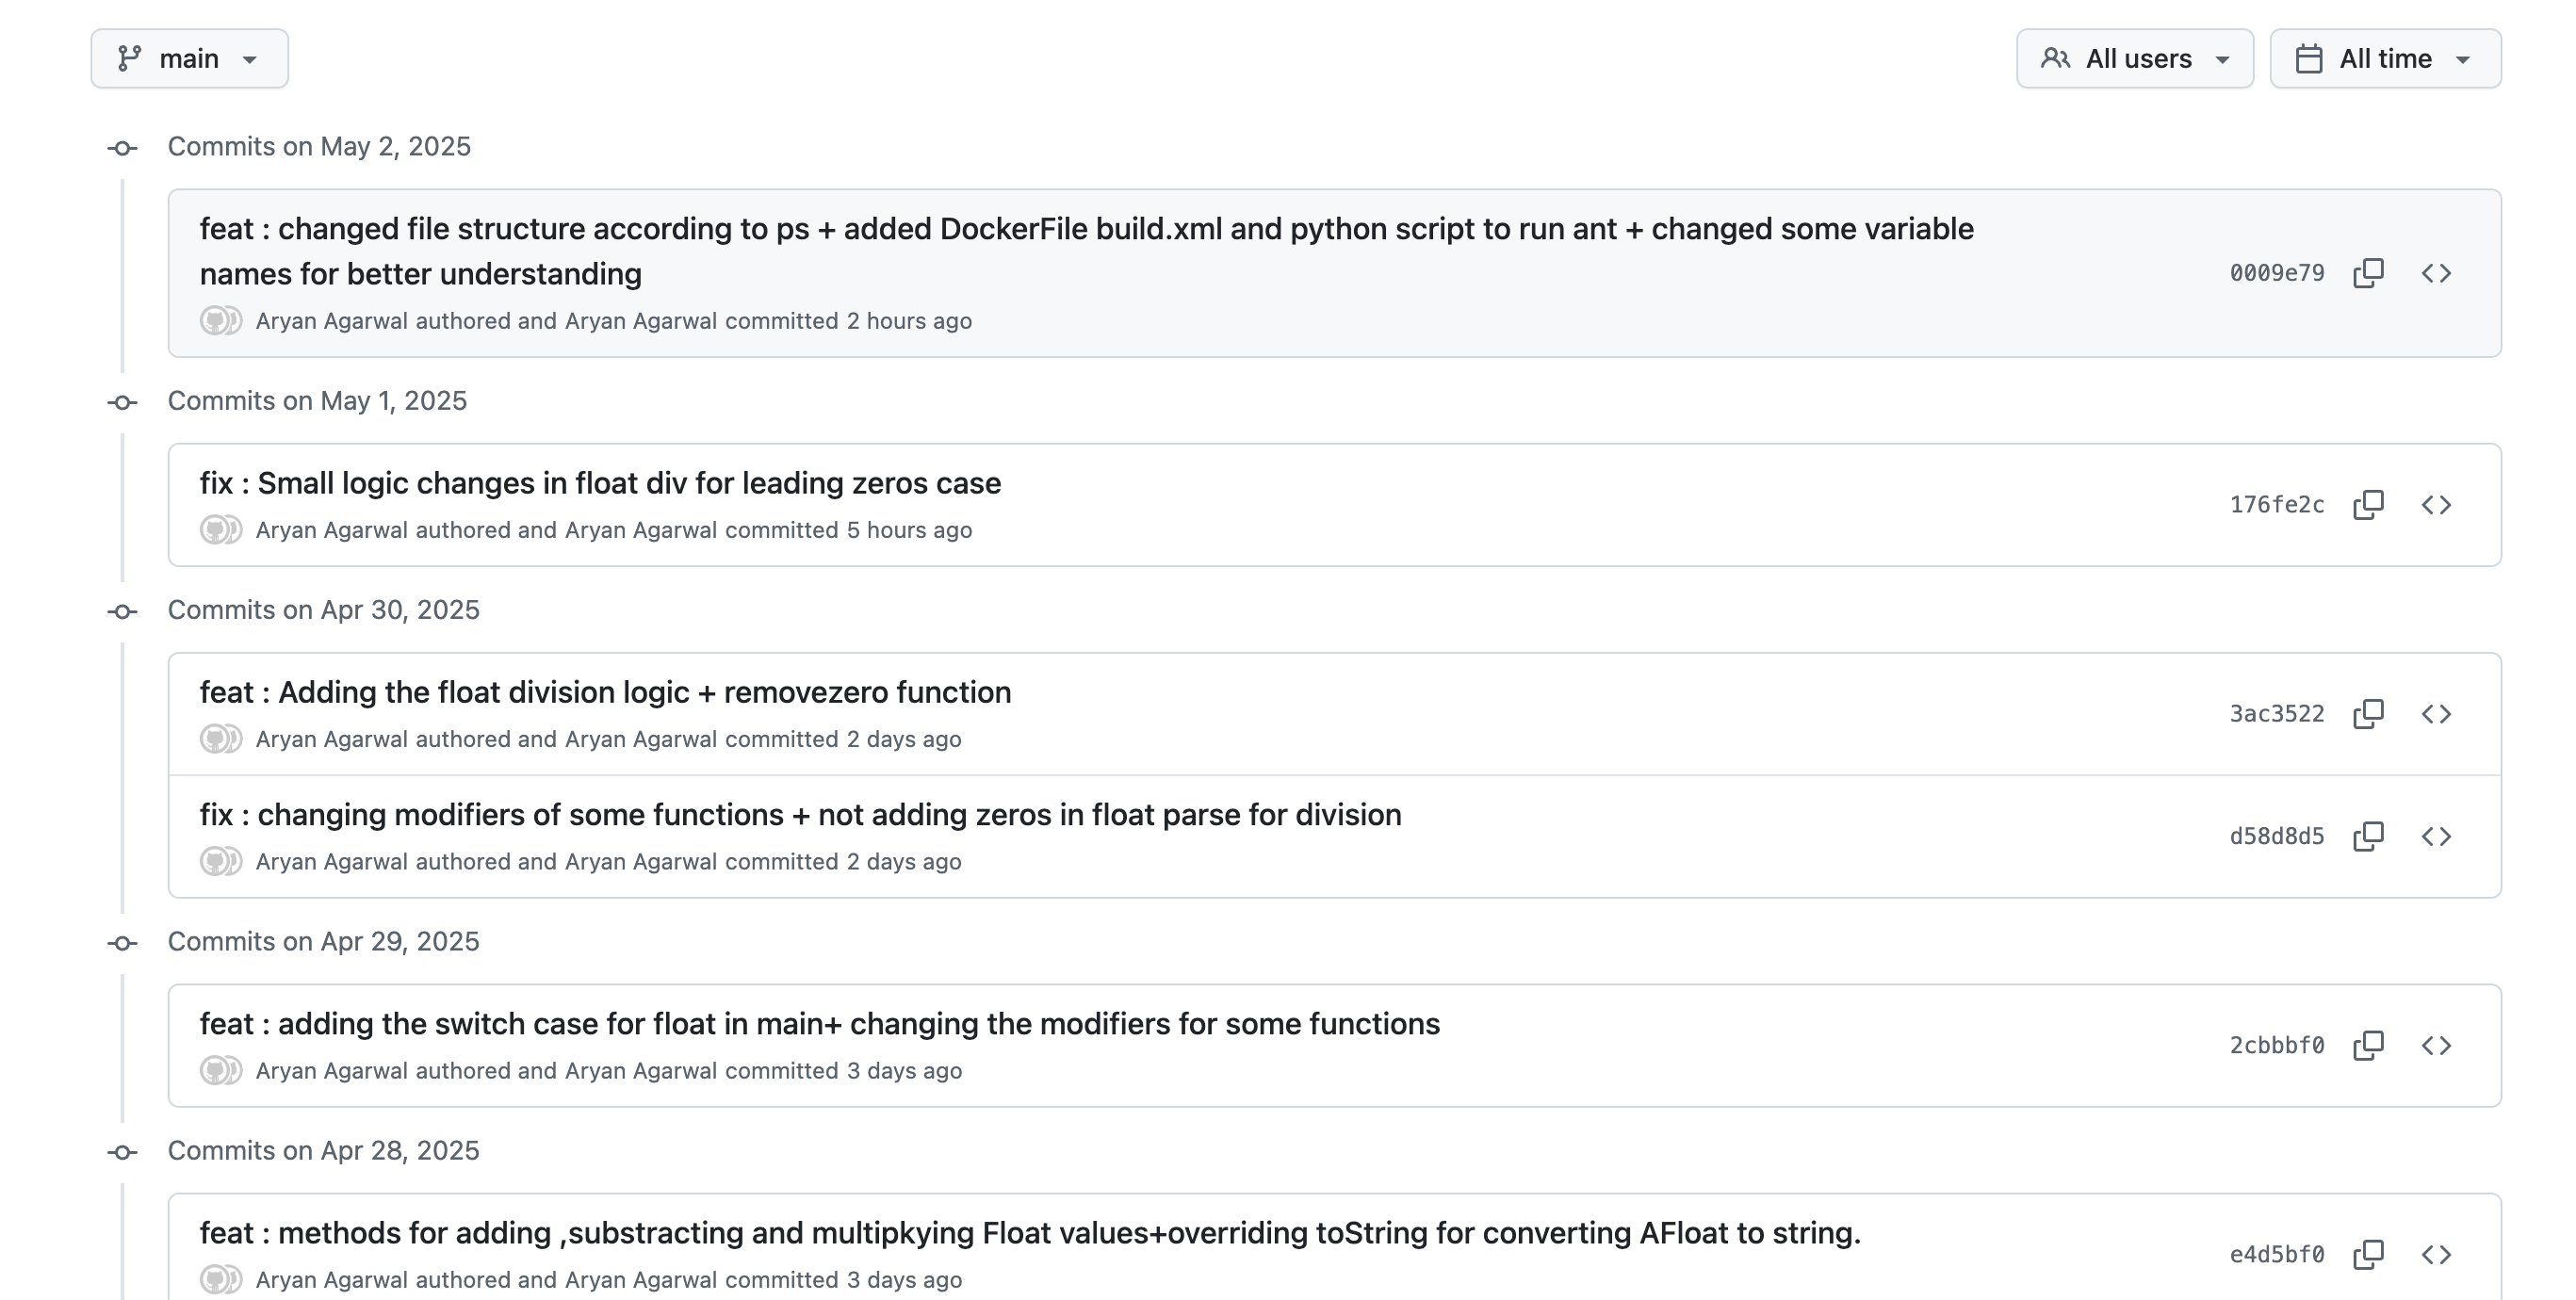
\includegraphics[width=0.8\textwidth]{images/p2.png}
\end{figure}

\section{What I Learned}
\begin{itemize}
  \item How to implement big-number math from scratch in Java.
  \item A lot about classes , methods, contructots etc in Java.
  \item How to cleanly separate sign logic from digit math.
  \item How to use Ant and a Python helper script for builds.
  \item How to use Docker and Git
\end{itemize}

\end{document}

